
\chapter{Results}
\label{ch:results}

The three implementations discussed in \cref{ch:direct_intersection,ch:tri_dexel,ch:point_cloud_based} have been tested on the scenes described in chapter \cref{ch:test_scenes}.
Each implementation has been benchmarked on the same machine, utilizing an Intel Core i7-3770 quad-core processor at \SI{3.4}{\giga\hertz} with \SI{16}{\gibi\byte} RAM.
All timings in this chapter are averaged over ten runs, unless stated otherwise.
The CPU utilization of each algorithm is shown as well.
The meshes reconstructed by each implementation at every scene have been rendered using MeshLab \cite{meshlab}.
Where appropriate, detailed renderings are shown to discuss special aspects of an implementation.
Finally, the number of created boundary edges is given for each reconstructed mesh as measured by MeshLab.

\section{Direct intersection}
\label{sec:direct_intersection_results}

The runtime and output size of the test runs of the direct intersection surface reconstruction are detailed in \Cref{tbl:direct_intersection_results}.
%
\begin{table}
	\centering
	\begin{tabular}{lrrrrr}
		scene          & SVs  & t\sub{in} & t\sub{out} & {time} \\
		\midrule
		cube2          &    1 & \SI{  0.8}{\kilo\nothing} & \SI{   1}{\kilo\nothing} & \SI{  1.0}{\milli\second}            \\
		cylinders\_d   &    1 & \SI{    7}{\kilo\nothing} & \SI{  10}{\kilo\nothing} & \SI{  6.0}{\milli\second}            \\
		cylinders      &    1 & \SI{    4}{\kilo\nothing} & \SI{   7}{\kilo\nothing} & \SI{  9.0}{\milli\second}            \\
		cylinder\_head &   20 & \SI{   80}{\kilo\nothing} & \SI{ 149}{\kilo\nothing} & \SI{229.0}{\milli\second}            \\
		impeller       & 2383 & \SI{ 6000}{\kilo\nothing} & \SI{1677}{\kilo\nothing} & \SI{ 21.0}{      \second}\phantom{m} \\
		impeller\_2    & 1191 & \SI{ 3000}{\kilo\nothing} & \SI{1296}{\kilo\nothing} & \SI{ 11.0}{      \second}\phantom{m} \\
		turbine        &  480 & \SI{16000}{\kilo\nothing} & \SI{ 752}{\kilo\nothing} & \SI{280.0}{      \second}\phantom{m} \\
	\end{tabular}
	\caption{
		Test results for the direct intersection surface extraction approach.
	}
	\label{tbl:direct_intersection_results}
\end{table}
%
The timings vary a lot from \SI{1}{\milli\second} for the simple cube2 scene up to \SI{280}{\second} for the turbine scene.
The runtime depends on multiple characteristics of the input.
The number of swept volumes increase the runtime linearly, as seen when comparing the timings of the impeller and impeller\_2 scene.
This consequence can also be derived from \cref{alg:direct_intersection} where the \textproc{DirectIntersection} function performs a pairwise reduction of all structures of a single cell, a linear operation.

All other parameters influence the runtime in less easily comprehensible ways.
The turbine scene for example has a little more than three times the triangles to process than the impeller scene and a lot less swept volumes, but requires more than ten times the computation time.
What causes the big difference in this case is mostly the triangle density per structure.
When dividing the number of totally stored triangles by the number of swept volumes, we can get a rough idea of the complexity of a single swept volume.
This number is roughly 2500 for the impeller scenes and 33000 for the turbine scene.
As the grid resolution is almost identical in these scenes, the parts of a swept volume assigned to each cell, \ie the structures, are substantially larger.

An increase in the number of triangles per structure, raises the runtime quadratically in several sub-algorithms.
Having a look on the basic structure of the direct intersection approach in \cref{alg:direct_intersection}, the \textproc{ClipStructure} and the \textproc{SplitTriangle} functions run linearly with the number of triangles per structure, whereas the \textproc{IntersectTriangle} and \textproc{IsTriangleInsideStructure} form nested loops on all triangles of the structure, \ie require quadratic time.
Considering the additional code required to increase numeric stability discussed in \cref{sec:numeric_improvements}, the collapsing of near points of a structure is also a quadratic operation.
The algorithms with quadratic runtime also light up in profiling sessions with \textproc{IntersectTriangle} consuming \SI{38}{\percent}, near points collapsing \SI{26}{\percent} and \textproc{IsTriangleInsideStructure} \SI{18}{\percent} of the total runtime.

The grid resolution affects the runtime by partitioning the whole problem into smaller parts.
A finer grid causes structures to be smaller and the output to contain fewer errors as cells contain fewer structures and triangles.
Especially the quadratic functions benefit from smaller structures.
However, as a consequence of a finer grid, more cells have to be processed in total.
As processing cells is a linear operation, \cf \cref{alg:direct_intersection}, increasing the grid resolution is usually beneficial.
Nevertheless, maintaining the grid and related data structures requires time and especially memory, thus restricting its granularity.
Resolutions between 100 and 150 cells in one dimensions usually proofed to be good choices for real world scenarios.

The amount of exploitable parallelism has already been discussed in \cref{sec:parallelization}.
The topmost loop of the \textproc{DirectIntersection} function has been parallelized in the implementation using Microsoft's Parallel Patterns Library (PPL) and the parallel\_for function which uses a scheduler implementing work stealing to balance the workload \cite{ppl_parallel_for}.
The CPU utilization during an single run of the direct intersection approach on the impeller scene is shown in \cref{fig:di_cpu}.
%
\begin{figure}
	\centering
	\begin{tikzpicture}
	\begin{axis}[
	width=0.95\textwidth,
	height=0.5\textwidth,
	xlabel={Wall clock time in \si{\second}},
	ylabel={CPU utilization in \si{\percent}},
	ymin=0,
	ymax=100,
	ytick={0,20,...,100},
	xtick={6,9,...,33}
	]
	\addplot table [x=time, y=utilization, col sep=comma]{spreadsheets/di_hq_impeller_cpu.csv};
	\end{axis}
	\end{tikzpicture}
	%\includegraphics[width=0.8\textwidth]{di_hq_impeller_cpu}
	\caption{
		CPU utilization during a run of the direct intersection algorithm to reconstruct the surface of the impeller scene.
		Measured using the profiler of Visual Studio 2013.
	}
	\label{fig:di_cpu}
\end{figure}
%
The CPU cores are almost perfectly utilized for the first 20 seconds.
Afterwards, the workload drops down to zero within the last three seconds of the run.
The PPL's default scheduler already works well, keeping all cores utilized for \SI{85}{\percent} of the runtime.
This slow drop at the end of the test run might be improved by employing a better scheduling strategy.
However, more complex scheduling usually also increases the parallelization overhead.
%
Concerning memory, the regular grid holding the impeller requires approximately \SI{600}{\mebi\byte} memory.
During the algorithm, \SI{300}{\mebi\byte} additional memory has been allocated, mostly for the temporary union structures and the buffer holding the resulting surface.

\Cref{fig:di_results} contains renderings of the resulting triangle meshes.
%
\begin{figure}
	\centering
	\begin{subfigure}[b]{0.34\textwidth}
		\centering
		\includegraphics[width=\textwidth]{di_cube2}
		\caption{cube2}
		\label{fig:di_cube2}
	\end{subfigure}
	\hspace{1cm}
	\begin{subfigure}[b]{0.34\textwidth}
		\centering
		\includegraphics[width=\textwidth]{di_cylinder_head}
		\caption{cylinder\_head}
		\label{fig:di_cylinder_head}
	\end{subfigure}
	\begin{subfigure}[b]{0.34\textwidth}
		\centering
		\includegraphics[width=\textwidth]{di_cylinders}
		\caption{cylinders}
		\label{fig:di_cylinders}
	\end{subfigure}
	\hspace{1cm}
	\begin{subfigure}[b]{0.34\textwidth}
		\centering
		\includegraphics[width=\textwidth]{di_cylinders_delaunay}
		\caption{cylinders\_d}
		\label{fig:di_cylinders_d}
	\end{subfigure}
	\begin{subfigure}[b]{0.34\textwidth}
		\centering
		\includegraphics[width=\textwidth]{di_hq_impeller}
		\caption{impeller}
		\label{fig:di_impeller}
	\end{subfigure}
	\hspace{1cm}
	\begin{subfigure}[b]{0.34\textwidth}
		\centering
		\includegraphics[width=\textwidth]{di_hq_impeller_2}
		\caption{impeller\_2}
		\label{fig:di_impeller_2}
	\end{subfigure}
	\begin{subfigure}[b]{0.33\textwidth}
		\centering
		\includegraphics[width=\textwidth]{di_turbine}
		\caption{turbine}
		\label{fig:di_turbine}
	\end{subfigure}
	\caption{
		Renderings of the result meshes after applying the direct intersection reconstruction approach on the selected test scenes in \cref{tbl:test_scenes}.
	}
	\label{fig:di_results}
\end{figure}
%
The cube2 scene has been extracted almost correctly.
All intersecting triangles have been properly split and retriangulated.
There is one small hole at one of the edges and a few falsely remaining ones at the bottom left of the cutting surface, \cf \cref{fig:di_cube2}.
These errors are due to a wrong outcome of the inside test, \cf \textproc{IsTriangleInsideStructure} in \cref{alg:triangle_inside_test}.
Nevertheless, the errors in the reconstructed surface are small and may be corrected manually using an appropriate 3D modeling tool, creating a closed mesh.

Both cylinder scenes delivered good results.
The variant with the small and thin triangles even resulted in an almost perfect surface with no holes and no leftover triangles.
Surprisingly, the other variant with the quality triangulation contained nine holes and one un-eliminated triangle.
This outcome is quite the opposite of what had been observed during the development of the algorithm.
In early stages, before the GTE library had been used for its excellent CDT, the core problem was the correct splitting of intersected triangles, which was much more stable on smaller and more regular triangles.
With the use of GTE, the numeric problems shifted from the CDT to the \textproc{IsTriangleInsideStructure} test.
The reason why smaller and more regular triangles entail a higher error rate in this test is not entirely clear.
The test is quite sensitive to the chosen target point of the structure used for casting the test ray.
Furthermore, a lot if ray-triangle intersections are performed where triangle normals are compared with the ray's direction, \cf details of \cref{alg:triangle_inside_test}.
All these tests are numerically unstable, if the ray is almost parallel to the tested triangles.
Assuming infinite precision, the tested triangle should always lie clearly inside or outside the structure it is tested against, otherwise there must have been an intersection and the triangle would have been split.
In practice, if an intersection is missed and the triangle spans the structure, or the tested triangle is almost degenerated and very close to the structure, errors may occur.

Concerning the more complex scenes, the impeller and turbine surfaces look quite good from a distance.
However, reviewing the details reveals numerous errors.
\Cref{fig:di_scenes_artifacts} shows two detailed views, one centered on a smaller blade of the impeller and one centered on a milling groove of the turbine.
%
\begin{figure}
	\centering
	\begin{subfigure}[b]{\textwidth}
		\centering
		\includegraphics[width=0.8\textwidth]{di_hq_impeller_detail}
		\caption{impeller}
		\label{fig:di_impeller_detail}
	\end{subfigure}\\
	\begin{subfigure}[b]{\textwidth}
		\centering
		\includegraphics[width=0.8\textwidth]{di_turbine_detail}
		\caption{turbine}
		\label{fig:di_turbine_detail}
	\end{subfigure}
	\caption{
		Renderings of selected areas from the impeller \subref{fig:di_impeller_detail} and turbine \subref{fig:di_turbine_detail} scene after applying the direct intersection reconstruction approach.
	}
	\label{fig:di_scenes_artifacts}
\end{figure}
%
Especially the impeller scene contains quite a lot of intersecting triangles and structures in each cell.
When zooming very close to the edges of a blade, several intersecting triangles can be seen which have not been split, probably due to errors when detecting the intersection lines.
These errors may then cause consequential errors in \eg the triangle inside test.
As the impeller's grid contains cells with up to 64 structures, small mistakes add up iteratively and may cause huge defects on the final surface.
Especially the cells which contain triangles from many swept volumes, \ie cells at the blade edges, suffer from this effect.
The triangle inside test still operates acceptably and the final surface does somehow resemble the surface of the machining result.
Nonetheless, the reconstructed surface contains a huge number of holes and boundaries as well as lots of intersecting triangles, \cf \cref{tbl:direct_intersection_results}.
Regarding the quality of the produced mesh, the result is probably worthless for subsequent tasks, like using it for simulations.

The turbine scene seems to have a similar problem.
Most of the intersections between stock and swept volume triangles have not been caught.
As the total number of swept volumes is relatively low compared to the impeller scene and only very few of them intersect each other, the surface errors are considerably smaller.
By deleting self-intersecting triangles from the outcome, an intelligent hole closing algorithm might be able to recover a closed surface, \eg an adaption of the ball-pivoting algorithm \cite{bpa}.

All extracted meshes in general have issues with neighboring triangles not having identical shared vertices.
The difference however is neglectable and can easily be corrected in a post processing step which merges close vertices, \eg using the Merge Close Vertices filter of MeshLab.
Furthermore, the result contains many T-vertices around intersected triangles, which result from clipping the triangles of a cell after the triangle-triangle intersections and retriangulations instead of before these two stages, \cf \cref{sec:clipping}.

\begin{table}
	\centering
	\begin{tabular}{l|r}
		scene          &  boundary edges         \\
		\midrule
		cube2          & \SI{ 75}{     \nothing} \\
		cylinders\_d   & \SI{ 69}{     \nothing} \\
		cylinders      & \SI{  1}{\kilo\nothing} \\ %   1078
		cylinder\_head & \SI{ 22}{\kilo\nothing} \\ %  22432
		impeller       & \SI{660}{\kilo\nothing} \\ % 659695
		impeller\_2    & \SI{326}{\kilo\nothing} \\ % 326171
		turbine        & \SI{402}{\kilo\nothing} \\ % 401917
	\end{tabular}
	\caption{
		Created boundary edges by the direct intersection surface extraction.
	}
	\label{tbl:direct_intersection_boundary edges}
\end{table}
%
The created boundary edges of the direct intersection reconstruction are listed in \cref{tbl:direct_intersection_results}.
These numbers are fairly high, especially at the real-world and complicated scenes.
However, these numbers specify the number of edges at a boundary, not the number of holes, which is considerably smaller.
In fact, most of the boundary edges in simpler scenes, \eg cylinders and cylinder\_head, are attributed to T-vertices.
Nevertheless, more complex scenes like the impeller or turbine truly contain an extensive amount of holes, as sceen in their detailed renderings, \cf \cref{fig:di_scenes_artifacts}.

\section{Tri-dexel}
\label{sec:tri_dexel_results}

Finally, the tri-dexel surface reconstruction approach described in this chapter has been tested on the scenes described in \cref{ch:test_scenes}.
A few different grid resolutions have been used, which are 50, 100, 200 and 400.
\Cref{tbl:tri_dexel_results} contains the runtime and output size of the test runs.
%
\begin{table}
	\begin{subtable}{\textwidth}
		\centering
		\begin{tabular}{l|rr|rr|rr|rr}
			resolution     & \multicolumn{2}{c}{50} & \multicolumn{2}{c}{100} & \multicolumn{2}{c}{200} & \multicolumn{2}{c}{400} \\
			scene          & t\sub{out} & time & t\sub{out} & time & t\sub{out} & time & t\sub{out} & time \\
			\midrule
			cube2          & \SI{55}{\kilo\nothing} & \SI{137}{\milli\second} & \SI{222}{\kilo\nothing} & \SI{1.1}{\second} & \SI{901}{\kilo\nothing} & \SI{10.5}{\second} & \SI{3.6}{\mega\nothing} & \SI{203}{\second} \\
			cylinders\_d   & \SI{33}{\kilo\nothing} & \SI{ 39}{\milli\second} & \SI{112}{\kilo\nothing} & \SI{0.3}{\second} & \SI{436}{\kilo\nothing} & \SI{ 2.1}{\second} & \SI{1.7}{\mega\nothing} & \SI{ 27}{\second} \\
			cylinders      & \SI{30}{\kilo\nothing} & \SI{ 34}{\milli\second} & \SI{112}{\kilo\nothing} & \SI{0.3}{\second} & \SI{435}{\kilo\nothing} & \SI{ 2.1}{\second} & \SI{1.7}{\mega\nothing} & \SI{ 26}{\second} \\
			cylinder\_head & \SI{74}{\kilo\nothing} & \SI{ 56}{\milli\second} & \SI{263}{\kilo\nothing} & \SI{0.4}{\second} & \SI{965}{\kilo\nothing} & \SI{ 2.9}{\second} & \SI{3.8}{\mega\nothing} & \SI{ 32}{\second} \\
			impeller       & \SI{76}{\kilo\nothing} & \SI{135}{\milli\second} & \SI{242}{\kilo\nothing} & \SI{0.6}{\second} & \SI{853}{\kilo\nothing} & \SI{ 3.3}{\second} & \SI{3.0}{\mega\nothing} & \SI{ 27}{\second} \\
			impeller\_2    & \SI{62}{\kilo\nothing} & \SI{ 95}{\milli\second} & \SI{195}{\kilo\nothing} & \SI{0.5}{\second} & \SI{696}{\kilo\nothing} & \SI{ 3.1}{\second} & \SI{2.5}{\mega\nothing} & \SI{ 31}{\second} \\
			turbine        & \SI{38}{\kilo\nothing} & \SI{179}{\milli\second} & \SI{162}{\kilo\nothing} & \SI{0.8}{\second} & \SI{629}{\kilo\nothing} & \SI{ 3.7}{\second} & \SI{2.3}{\mega\nothing} & \SI{ 21}{\second} \\
		\end{tabular}
		\caption{
			without cell slicing.
		}
		\label{tbl:tri_dexel_results_no_slicing}
	\end{subtable}
	\bigskip\\
	\begin{subtable}{\textwidth}
		\centering
		\begin{tabular}{l|rr|rr|rr|rr}
			resolution     & \multicolumn{2}{c}{50} & \multicolumn{2}{c}{100} & \multicolumn{2}{c}{200} & \multicolumn{2}{c}{400} \\
			scene          & t\sub{out} & time & t\sub{out} & time & t\sub{out} & time & t\sub{out} & time \\
			\midrule
			cube2          & \SI{55}{\kilo\nothing} & \SI{ 138}{\milli\second} & \SI{222}{\kilo\nothing} & \SI{1.1}{\second} & \SI{901}{\kilo\nothing} & \SI{10.5}{\second} & \SI{3.6}{\mega\nothing} & \SI{198}{\second} \\
			cylinders\_d   & \SI{33}{\kilo\nothing} & \SI{  38}{\milli\second} & \SI{113}{\kilo\nothing} & \SI{0.3}{\second} & \SI{436}{\kilo\nothing} & \SI{ 2.1}{\second} & \SI{1.7}{\mega\nothing} & \SI{ 27}{\second} \\
			cylinders      & \SI{30}{\kilo\nothing} & \SI{  33}{\milli\second} & \SI{112}{\kilo\nothing} & \SI{0.3}{\second} & \SI{435}{\kilo\nothing} & \SI{ 2.1}{\second} & \SI{1.7}{\mega\nothing} & \SI{ 26}{\second} \\
			cylinder\_head & \SI{81}{\kilo\nothing} & \SI{ 102}{\milli\second} & \SI{276}{\kilo\nothing} & \SI{0.5}{\second} & \SI{988}{\kilo\nothing} & \SI{ 3.0}{\second} & \SI{3.8}{\mega\nothing} & \SI{ 32}{\second} \\
			impeller       & \SI{82}{\kilo\nothing} & \SI{ 743}{\milli\second} & \SI{252}{\kilo\nothing} & \SI{1.8}{\second} & \SI{872}{\kilo\nothing} & \SI{ 6.3}{\second} & \SI{3.0}{\mega\nothing} & \SI{ 51}{\second} \\
			impeller\_2    & \SI{66}{\kilo\nothing} & \SI{ 358}{\milli\second} & \SI{200}{\kilo\nothing} & \SI{1.0}{\second} & \SI{708}{\kilo\nothing} & \SI{ 3.9}{\second} & \SI{2.5}{\mega\nothing} & \SI{ 38}{\second} \\
			turbine        & \SI{47}{\kilo\nothing} & \SI{3068}{\milli\second} & \SI{180}{\kilo\nothing} & \SI{8.1}{\second} & \SI{657}{\kilo\nothing} & \SI{23.5}{\second} & \SI{2.3}{\mega\nothing} & \SI{145}{\second} \\
		\end{tabular}
		\caption{
			with cell slicing.
		}
		\label{tbl:tri_dexel_results_slicing}
	\end{subtable}
	\caption{
		Test results for the tri-dexel surface extraction approach without and with one recursion of cell slicing.
	}
	\label{tbl:tri_dexel_results}
\end{table}
%
Concerning the number of triangles outputted by the reconstruction, t\sub{out}, two trends are observable.
At first, when the same resolution is used, t\sub{out} is roughly equal for all scene, since t\sub{out} does not depend on the amount of triangles needed by the VML to describe the scene.
Actually, only the shape of the scene has an impact on this value.
Taking a perfect cube for example and a resolution of 50, each of the six cube side would be sampled by $50\times50$ rays, resulting in $6 \times 50 \times 50 = \SI{15}{\kilo\nothing}$ surface points.
This number is a good approximation of the number of boundary cells too.
Each boundary cell then contains a loop of four vertices, triangulated into a fan with four triangles, yielding $\SI{15}{\kilo\nothing} \times 4 = \SI{60}{\kilo\nothing}$ total triangles.
Depending on the feature richness and size of the scene along all axes, the number of extracted triangles will be around this number, which is perfectly observable in the first column of \cref{tbl:tri_dexel_results}.

The second finding is that t\sub{out} increases quadratically with the resolution parameter.
This correlation stems from the fact that the resolution is applied to both sides of the raycasted dexel image, thereby increasing the number of rays and estimated boundary cells quadratically.
The rows of the results without cell slicing prove this statement, although scenes with richer features, \eg cylinder\_head and impeller, do not follow this rule as closely as flatter scenes, \eg cube2 and cylinders.
The results with cell slicing are less representative for this observation.
The reason is the adaptivity of the algorithm.
Lower resolutions tend to produce more irregular cells, as the grid resolution is too coarse to capture a model's features.
Therefore, a lot more sub cells are created.
Consequently, the resolution and triangle count is automatically increased in feature rich areas.
The finer the initial resolution is, the lesser this effect manifests itself.

Regarding the runtime of the extraction, the relation to the resolution is a bit more difficult.
To start with, the basic algorithms used throughout the tri-dexel extraction are either of quadratic or cubic complexity.
The raycast is asymptotically $\mathcal{O}(n^2)$, whereas the cell processing is $\mathcal{O}(n^3)$ and the dexel assignment somewhere in between, $\mathcal{O}(n^2p)$ which $p$ being the average number of grid points spanned by segments on a dexel.
However, cell processing is only intensive on boundary cells, which only grow quadratically with the resolution.
The tri-dexel's runtime is therefore somewhere between $\mathcal{O}(n^2)$ and $\mathcal{O}(n^3)$.
To some degree, this hypothesis is observable at the data in \cref{tbl:tri_dexel_results}, where the increase in runtime is somewhere around five to seven times when the resolution is doubled.
The cube2 scene seems to be an exception to this rule.
However, the cube2 scene, by being completely cubic, also results in a tri-dexel grid with the most cells possible for a given resolution.
As collecting these cells is quite expensive, this scene has a higher, memory-related overhead than most of the other scenes which have a smaller extent along one of the axes.

Comparing the version of the algorithm with and without cell slicing, a considerable difference has been measured.
The triangle count of the resulting mesh is usually a bit higher when reconstructed with cell slicing, as slicing locally increases the cell and triangle density.
By contrast, the runtime changes significantly when cell slicing is enabled.
The answer to this vast increase, especially in feature rich scenes like impeller and turbine, is given by profiling.
The functions doing most individual work\footnote{
	Functions having the most exclusive samples, \ie samples where the execution was inside the body of a function when the sample was taken, without samples of functions called from the body.}
are all found within the raycasting component.
They are \textproc{IntersectCell} with \SI{24}{\percent}, \textproc{IntersectTriangle} with \SI{17}{\percent} and a operating system function handling heap allocations with \SI{9}{\percent}.
Further interesting is the stage of the algorithm at which these functions are heavily used.
Apart from the initial raycast, these functions still consume half of the available CPU power.
The reason therefore is the high cost of traversing rays through the VML's regular grid and intersecting them with the encountered triangles.
Now, every time a tri-dexel cell is sliced, tri-dexel images have to be recreated for the resulting sub cells, requiring further raycasts.
The performance of the raycast itself depends mostly on the number of triangles per cell, as all these triangles have to be pulled from RAM and tested for intersection.
Considering the triangle count distributions of the test scenes in \cref{fig:histograms}, it is obvious why the impeller and especially the turbine require a far longer runtime than other scenes.

Parallelization has already been discussed in \cref{sec:tri_dexel_parallelization} and has been applied where suitable, again using Microsoft's PPL and the parallel\_for primitive \cite{ppl_parallel_for}.
The CPU utilization during a single run of the tri-dexel surface extraction of the impeller scene with a grid resolution of 200 is shown in \cref{fig:td_hq_impeller_cpu}.
%
\begin{figure}
	\centering
	\begin{tikzpicture}
	\begin{axis}[
	width=0.95\textwidth,
	height=0.5\textwidth,
	xlabel={Wall clock time in \si{\second}},
	ylabel={CPU utilization in \si{\percent}},
	ymin=0,
	ymax=100,
	ytick={0,20,...,100},
	xtick={7,8,...,16}
	]
	\addplot table [x=time, y=utilization, col sep=comma]{spreadsheets/td_hq_impeller_cpu.csv};
	\end{axis}
	\end{tikzpicture}
	%\includegraphics[width=0.9\textwidth]{images/td_hq_impeller_cpu}
	\caption{
		CPU utilization during a run of the tri-dexel algorithm with a grid resolution of 200 along the longest axis, all features enabled, reconstructing the surface of the impeller scene.
		Measured using the profiler of Visual Studio 2013.
	}
	\label{fig:td_hq_impeller_cpu}
\end{figure}
%
The extraction starts by performing a raycast on the VML's data model.
It takes some time in the beginning until the CPU reaches full utilization.
The profiler mostly highlights memory intensive operations during this time, such as pulling the triangles from RAM and allocations.
After 1 - 1.5 seconds, the raycast has finished and the construction of the tri-dexel grid starts.
Again, this process requires a lot of memory allocations, which are serialized by the operating system, causing the utilization to drop slightly.
This drop includes the aggregation of data to form isolated cells, which is memory intensive as well.

Processing cells starts right away after the first cells are available.
At this point the CPU again reaches maximum utilization for almost the complete extraction, as the granularity of the parallelization is quite fine, \ie lots of cells are available to saturate all cores.
However, as fully occupied and non-occupied cells do not need any processing, only boundary cells contribute to the surface, the intensity of a work item varies.
In the last second, triangulation has been finished for almost all cells.
Most of the work left is freeing allocated resources, which takes quite a while and is again serialized by the operating system, causing the utilization to drop drastically for the last second.

Regarding the allocated memory, in addition to the VML's regular grid holding the impeller scene in \SI{600}{\mebi\byte}, the tri-dexel algorithm requires approximately \SI{425}{\mebi\byte} additional memory at a grid resolution of 400, mostly for storing the dexel images, grid point occupancies and grid edges with their segments.
On third of the memory is allocated before the raycast, another third during the raycast and the last third when building the tri-dexel grid.
While cells are processed, cell data is aggregated, regularized, triangulated and immediately freed again.
Therefore, the memory consumption remains almost constant during the further execution after the grid construction.

\Cref{fig:di_results} contains renderings of the resulting triangle meshes.
%
\begin{figure}
	\centering
	\begin{subfigure}[b]{0.34\textwidth}
		\centering
		\includegraphics[width=\textwidth]{td_cube2}
		\caption{cube2}
		\label{fig:td_cube2}
	\end{subfigure}
	\hspace{1cm}
	\begin{subfigure}[b]{0.34\textwidth}
		\centering
		\includegraphics[width=\textwidth]{td_cylinder_head}
		\caption{cylinder\_head}
		\label{fig:td_cylinder_head}
	\end{subfigure}
	\begin{subfigure}[b]{0.34\textwidth}
		\centering
		\includegraphics[width=\textwidth]{td_cylinders}
		\caption{cylinders}
		\label{fig:td_cylinders}
	\end{subfigure}
	\hspace{1cm}
	\begin{subfigure}[b]{0.34\textwidth}
		\centering
		\includegraphics[width=\textwidth]{td_cylinders_d}
		\caption{cylinders\_d}
		\label{fig:td_cylinders_delaunay}
	\end{subfigure}
	\begin{subfigure}[b]{0.34\textwidth}
		\centering
		\includegraphics[width=\textwidth]{td_hq_impeller}
		\caption{impeller}
		\label{fig:td_hq_impeller}
	\end{subfigure}
	\hspace{1cm}
	\begin{subfigure}[b]{0.34\textwidth}
		\centering
		\includegraphics[width=\textwidth]{td_hq_impeller_2}
		\caption{impeller\_2}
		\label{fig:td_hq_impeller_2}
	\end{subfigure}
	\begin{subfigure}[b]{0.33\textwidth}
		\centering
		\includegraphics[width=\textwidth]{td_turbine}
		\caption{turbine}
		\label{fig:td_turbine}
	\end{subfigure}
	\caption{
		Renderings of the result meshes after applying the tri-dexel reconstruction approach with a grid resolution of 400 on the selected test scenes in \cref{tbl:test_scenes}.
	}
	\label{fig:td_results}
\end{figure}
%
The cube2 scene has been extracted flawlessly.
All features, \ie edges and corners, of the cube have been perfectly reconstructed.
The only flaw is the high number of triangles outputted, \cf \cref{tbl:tri_dexel_results}.
However, this number is steered by the dexel grid's resolution and may be set very low for this simple scene.
Furthermore, an additional post-processing pass may be used to recombine adjacent triangles facing in the same direction\footnote{Third-party tools may also be used to manually reduce the triangle count, \eg MeshLab's Quadric Edge Collapse Decimation filter.}.

Both of the cylinders scenes deliver great results as well.
They show perfect edges at the stock as well as at the intersection with the smaller cylindrical swept volume.
However, the cylinders scene, on the top and bottom side, contains a small notch beside the hole drilled out.
This small error is the result of a numeric miscalculation in the raycaster, due to the thin triangles, which could not correctly identify the surface entry and exit for two incident rays.
Therefore, two dexels are completely empty at this location.
This case is handled by regularization rule three, which creates small segments at the grid's occupied points where the two dexels are empty.
The cylinders\_d scene does not contain any notches or other errors.
Concerning the feature reconstruction capabilities, the algorithm also managed to recover the shape of the original triangulation, which is clearly visible at the side of the stock and at the drilled hole.

Furthermore, the impeller scenes have been extracted very well too.
\Cref{fig:td_hq_impeller_details} shows two detailed renderings.
%
\begin{figure}
	\centering
	\begin{subfigure}[b]{0.49\textwidth}
		\centering
		\includegraphics[width=\textwidth]{td_hq_impeller_drillings}
		\caption{impeller drillings}
		\label{fig:td_hq_impeller_drillings}
	\end{subfigure}
	\begin{subfigure}[b]{0.49\textwidth}
		\centering
		\includegraphics[width=\textwidth]{td_hq_impeller_blades}
		\caption{impeller blades}
		\label{fig:td_hq_impeller_blades}
	\end{subfigure}
	\caption{
		Details of the impeller scene extracted using the tri-dexel approach with a grid resolution of 400.
	}
	\label{fig:td_hq_impeller_details}
\end{figure}
%
The drillings in the middle resemble the cylindrical swept volumes perfectly, \cf \cref{fig:td_hq_impeller_drillings}.
The impeller's blades have sharp edges and, between them, even the rills of the single swept volumes are slightly visible, \cf \cref{fig:td_hq_impeller_blades}.
Nonetheless, similarly to the cylinders scene, several numeric issues occurred during the dexel image creation by the raycaster, resulting in numerous notches at the surface.

Finally, the turbine scene looks good as well.
However, as the turbine's grooves contain mostly concave features, a sufficient resolution is required to capture the scene's small peculiarities.
\Cref{fig:td_grooves} shows renderings of a detailed view on one of the turbine's grooves in different resolutions.
%
\begin{figure}
	\centering
	\begin{subfigure}[b]{0.24\textwidth}
		\centering
		\includegraphics[width=\textwidth]{td_turbine_groove_50}
		\caption{50}
		\label{fig:td_turbine_groove_50}
	\end{subfigure}
	\begin{subfigure}[b]{0.24\textwidth}
		\centering
		\includegraphics[width=\textwidth]{td_turbine_groove_100}
		\caption{100}
		\label{fig:td_turbine_groove_100}
	\end{subfigure}
	\begin{subfigure}[b]{0.24\textwidth}
		\centering
		\includegraphics[width=\textwidth]{td_turbine_groove_200}
		\caption{200}
		\label{fig:td_turbine_groove_200}
	\end{subfigure}
	\begin{subfigure}[b]{0.24\textwidth}
		\centering
		\includegraphics[width=\textwidth]{td_turbine_groove_400}
		\caption{400}
		\label{fig:td_turbine_groove_400}
	\end{subfigure}
	\caption{
		Detailed renderings with the same perspective of a groove of the turbine scene.
		The meshes were created using the tri-dexel reconstruction algorithm with the grid resolutions 50, 100, 200 and 400.
	}
	\label{fig:td_grooves}
\end{figure}
%
At a resolution of 50, the groove itself is spanned by a bit of geometry.
Doubling the resolution lets the tri-dexel algorithm reconstruct the groove but leaves some geometry left in the wavy sides of the groove.
Increasing the level of detail to a resolution of 200 already retrieves a quite good surface with only a few missing subtleties at the tips of the waves.
These are finally reconstructed using a resolution of 400.
Nonetheless, a few errors still remain due to irregularities on the dexel image caused by misjudgments of the raycaster.

Concluding, all extracted meshes offer great detail.
Especially convex features like sharp corners and edges are retrieved almost perfectly.
Concave features, like the ones of the turbine, seem a bit harder to reconstruct and require an appropriate resolution.

Without using cell slicing, all meshes are manifold, closed and orientable.
Enhancing the tri-dexel approach by slicing irregular cells greatly reduces dropping valuable information during regularization, resulting in far better refined features.
\Cref{fig:td_features_and_cell_slicing} shows the difference of the reconstructed mesh when using no refinement/feature reconstruction, when using feature reconstruction and when using feature reconstruction and cell slicing.
%
\begin{figure}
	\centering
	\begin{subfigure}[b]{0.67\textwidth}
		\centering
		\includegraphics[width=\textwidth]{td_cylinder_head_drilling_no_features}
		\caption{no feature reconstruction}
		\label{fig:td_cylinder_head_drilling_no_features}
	\end{subfigure}
	\bigskip\\
	\begin{subfigure}[b]{0.67\textwidth}
		\centering
		\includegraphics[width=\textwidth]{td_cylinder_head_drilling_features}
		\caption{feature reconstruction}
		\label{fig:td_cylinder_head_drilling_features}
	\end{subfigure}
	\bigskip\\
	\begin{subfigure}[b]{0.67\textwidth}
		\centering
		\includegraphics[width=\textwidth]{td_cylinder_head_drilling_cell_slicing}
		\caption{feature reconstruction and cell slicing}
		\label{fig:td_cylinder_head_drilling_cell_slicing}
	\end{subfigure}
	\caption{
		Details of the cylinder\_head scene rendered with the same perspective.
		The renderings show the effects of refinement, feature reconstruction and cell slicing.
		The meshes have been extracted using the tri-dexel approach at a grid resolution of 100.
	}
	\label{fig:td_features_and_cell_slicing}
\end{figure}
%
Without feature reconstruction, almost no edges are reconstructed correctly.
This is very well observable at drilling and the flat surface around it.
Also the edges of the cylinder\_head's fins lack sharpness.
Enabling feature reconstruction, \cf \cref{sec:tri_dexel_refinement}, achieves a lot of correctness by using the normal information of the dexel image to calculate good intermediate/feature points and apex vertices.
In addition to the feature reconstruction, the cell slicing strategy, \cf \cref{sec:tri_dexel_cellslicing}, finally manages to also capture thin features, which were previously thrown away by the regularization.

Although improving the outcome significantly, slicing cells is dangerous.
It may create holes and T-vertices in the mesh, at the border between regular cells and sliced cells, making the mesh orientable but not manifold and closed.
\Cref{fig:td_cylinder_head_issues} shows these issues by the example of the outmost rip of the cylinder\_head.
%
\begin{figure}
	\centering
	\begin{subfigure}[b]{0.49\textwidth}
		\centering
		\includegraphics[width=\textwidth]{td_cylinder_head_t_vertex}
		\caption{t-vertices}
		\label{fig:td_cylinder_head_t_vertex}
	\end{subfigure}
	\begin{subfigure}[b]{0.49\textwidth}
		\centering
		\includegraphics[width=\textwidth]{td_cylinder_head_hole}
		\caption{hole}
		\label{fig:td_cylinder_head_hole}
	\end{subfigure}
	\caption{
		Details of the cylinder\_head scene.
		Boundary edges are marked in green.
		The renderings show the creation of T-vertices and holes at the border of normal and sliced cells.
		The hole is created at the border of a cell and a sliced cell, which is discussed in \cref{fig:tri_dexel_hole_creation}.
		The meshes have been extracted using the tri-dexel approach with cell slicing at a grid resolution of 100.
	}
	\label{fig:td_cylinder_head_issues}
\end{figure}
%
Still, these holes are usually thin and closable by a post processing step.
If all T-vertices are also fixed, \eg by splitting triangles at the edge spanning the T-vertex, meshes created with cell slicing enabled may still be converted into a manifold and closed result.

\Cref{tbl:tri_dexel_boundary edges} contains the number of boundary edges for the tested scenes and resolutions and the tri-dexel variant using cell slicing.
%
\begin{table}
	\centering
	\begin{tabular}{l|r|r|r|r}
		scene          & \multicolumn{4}{|c}{resolution} \\
		&   50 &  100 &  200 &   400 \\
		\midrule
		cube2          &    0 &    0 &    0 &     0 \\
		cylinders\_d   &    0 &  128 &  238 &   846 \\
		cylinders      &    0 &    0 &    0 &     0 \\
		cylinder\_head &  871 & 1880 & 4136 &  4966 \\
		impeller       & 1129 & 2380 & 4654 & 11940 \\
		impeller\_2    &  574 & 1191 & 3033 &  6050 \\
		turbine        & 2006 & 3703 & 7181 & 13803 \\
	\end{tabular}
	\caption{
		Created boundary edges by the tri-dexel surface extraction using cell-slicing and the test scenes described in \cref{tbl:test_scenes}.
		The meshes created without cell-slicing do not contain boundary edges.
	}
	\label{tbl:tri_dexel_boundary edges}
\end{table}
%
These numbers are smaller than the ones produced by the direct intersection approach discussed in \cref{ch:direct_intersection}, \cf \cref{tbl:direct_intersection_results}.
The cube2 and cylinders scene even contain no boundary edges at all, as no cells have been sliced.
The reason therefore is that the geometry of both scenes is completely convex, resulting in very regular dexel images with long dexels typically spanning the whole workpiece.
The cylinders\_d's triangulation, compared with the cylinders', for example is slightly concave at the lateral surface.
Thus, close rays along these surfaces alternatingly enter and exit the surface, sometimes yielding short dexel segments which lead to irregular edges later.

The more complex scenes produce a larger number of boundary edges, mostly attributed to T-vertices, although the results show, that the number of boundaries is not related to the scene's input triangle or swept volume count, \cf \cref{tbl:test_scenes}.
The number of boundaries is directly related to the number of irregular cells, which depends on the feature richness, \ie the shape, of the workpiece.
The impeller\_2 scene, for example, contains roughly half as much feature-rich geometry as the impeller scene.
In contrast, the cylinder\_head, despite consisting of two orders of magnitude less swept volumes as the impeller, still produces a third of the impeller's boundary edge count.

Concerning the scenes themselves, the cylinder\_head creates almost all irregular cells and boundaries at the sharp edges of the fins, where subdivision is vital to extract these features.
The impeller scene contains its boundary vertices distributed equally over the machined area.
Finally, the turbine suffers a lot from numerical issues at the rays parallel and to the stock surface which are tinily underneath it, continually entering and exiting the flat surface.
The sliced cells are again irregular and caught by the recursion limit of the cell slicing algorithm.


\section{Point cloud based}
\label{sec:point_cloud_results}

The point cloud creation and the subsequent reconstruction using the BPA discussed in \cref{sec:point_cloud_reconstruction} have been benchmarked for the test scenes described in \cref{ch:test_scenes}.
Analogously to the tri-dexel benchmarks, the resolutions 50, 100, 200 and 400 have been used for the raycaster creating the point clouds.
\Cref{tbl:point_cloud_results} contains the runtime and output size of the created point clouds.
%
\begin{table}
	\centering
	\begin{tabular}{l|rr|rr|rr|rr}
		resolution     & \multicolumn{2}{c}{50} & \multicolumn{2}{c}{100} & \multicolumn{2}{c}{200} & \multicolumn{2}{c}{400} \\
		scene          & p\sub{out} & time & p\sub{out} & time & p\sub{out} & time & p\sub{out} & time \\
		\midrule
		cube2          & \SI{14}{\kilo\nothing} & \SI{  3}{\milli\second} & \SI{56}{\kilo\nothing} & \SI{ 12}{\milli\second} & \SI{226}{\kilo\nothing} & \SI{  47}{\milli\second} & \SI{907}{\kilo\nothing} & \SI{ 187}{\milli\second} \\
		cylinders\_d   & \SI{ 7}{\kilo\nothing} & \SI{  5}{\milli\second} & \SI{27}{\kilo\nothing} & \SI{ 17}{\milli\second} & \SI{108}{\kilo\nothing} & \SI{  63}{\milli\second} & \SI{436}{\kilo\nothing} & \SI{ 247}{\milli\second} \\
		cylinders      & \SI{ 7}{\kilo\nothing} & \SI{  3}{\milli\second} & \SI{26}{\kilo\nothing} & \SI{ 11}{\milli\second} & \SI{107}{\kilo\nothing} & \SI{  41}{\milli\second} & \SI{433}{\kilo\nothing} & \SI{ 161}{\milli\second} \\
		cylinder\_head & \SI{15}{\kilo\nothing} & \SI{  7}{\milli\second} & \SI{60}{\kilo\nothing} & \SI{ 23}{\milli\second} & \SI{242}{\kilo\nothing} & \SI{  86}{\milli\second} & \SI{976}{\kilo\nothing} & \SI{ 335}{\milli\second} \\
		impeller       & \SI{11}{\kilo\nothing} & \SI{ 99}{\milli\second} & \SI{46}{\kilo\nothing} & \SI{353}{\milli\second} & \SI{184}{\kilo\nothing} & \SI{1118}{\milli\second} & \SI{744}{\kilo\nothing} & \SI{3813}{\milli\second} \\
		impeller\_2    & \SI{ 9}{\kilo\nothing} & \SI{ 54}{\milli\second} & \SI{38}{\kilo\nothing} & \SI{193}{\milli\second} & \SI{155}{\kilo\nothing} & \SI{ 600}{\milli\second} & \SI{625}{\kilo\nothing} & \SI{2037}{\milli\second} \\
		turbine        & \SI{ 7}{\kilo\nothing} & \SI{165}{\milli\second} & \SI{31}{\kilo\nothing} & \SI{650}{\milli\second} & \SI{132}{\kilo\nothing} & \SI{2509}{\milli\second} & \SI{532}{\kilo\nothing} & \SI{9610}{\milli\second} \\
	\end{tabular}
	\caption{
		Test results for the point cloud creation.
	}
	\label{tbl:point_cloud_results}
\end{table}
%
Three trends, similarly to the results of the tri-dexel reconstruction in \cref{tbl:tri_dexel_results}, are also observable here.
Firstly, the number of created points p\sub{out} for a given resolution is again similar for all scenes.
Secondly, p\sub{out} increases quadratically with the resolution.
Thirdly, also the runtime increases quadratically with the resolution.
The reasons is the asymptotic complexity of $\mathcal{O}(n^2)$ of the raycaster, which is discussed in more detail in \cref{sec:tri_dexel_results}.
Furthermore, the dependency of the runtime on the scene's complexity as well as parallelization, CPU and memory consumption is also discussed there.

Concerning subsequent surface reconstruction algorithms, \cref{tbl:bpa_results} contains the mesh sizes and timings for the VML's BPA implementation.
The ball's radius is derived from the raycasting resolution and set to 1.5 times the diameter of a cell of the sampling grid created by three axis aligned raycasts.
%
\begin{table}
	\centering
	\begin{tabular}{l|rrr|rrr}
		resolution     & \multicolumn{3}{c}{50} & \multicolumn{3}{c}{100} \\
		scene          & p\sub{in} & t\sub{out} & time & p\sub{in} & t\sub{out} & time \\
		\midrule
		cube2          & \SI{14}{\kilo\nothing}& \SI{27}{\kilo\nothing} & \SI{53}{\milli\second} & \SI{56}{\kilo\nothing} & \SI{111}{\kilo\nothing} & \SI{222}{\milli\second} \\
		cylinders\_d   & \SI{ 7}{\kilo\nothing}& \SI{13}{\kilo\nothing} & \SI{22}{\milli\second} & \SI{27}{\kilo\nothing} & \SI{ 53}{\kilo\nothing} & \SI{ 95}{\milli\second} \\
		cylinders      & \SI{ 7}{\kilo\nothing}& \SI{13}{\kilo\nothing} & \SI{22}{\milli\second} & \SI{26}{\kilo\nothing} & \SI{ 53}{\kilo\nothing} & \SI{ 94}{\milli\second} \\
		cylinder\_head & \SI{15}{\kilo\nothing}& \SI{27}{\kilo\nothing} & \SI{60}{\milli\second} & \SI{60}{\kilo\nothing} & \SI{110}{\kilo\nothing} & \SI{223}{\milli\second} \\
		impeller       & \SI{11}{\kilo\nothing}& \SI{20}{\kilo\nothing} & \SI{48}{\milli\second} & \SI{46}{\kilo\nothing} & \SI{ 91}{\kilo\nothing} & \SI{200}{\milli\second} \\
		impeller\_2    & \SI{ 9}{\kilo\nothing}& \SI{17}{\kilo\nothing} & \SI{36}{\milli\second} & \SI{38}{\kilo\nothing} & \SI{ 76}{\kilo\nothing} & \SI{161}{\milli\second} \\
		turbine        & \SI{ 7}{\kilo\nothing}& \SI{ 9}{\kilo\nothing} & \SI{20}{\milli\second} & \SI{31}{\kilo\nothing} & \SI{ 53}{\kilo\nothing} & \SI{142}{\milli\second} \\
		
		\multicolumn{1}{l}{\bigskip} \\
		
		resolution     & \multicolumn{3}{c}{200} & \multicolumn{3}{c}{400} \\
		scene          & p\sub{in} & t\sub{out} & time & p\sub{in} & t\sub{out} & time \\
		\midrule
		cube2          & \SI{226}{\kilo\nothing}& \SI{449}{\kilo\nothing} & \SI{1022}{\milli\second} & \SI{907}{\kilo\nothing}& \SI{1807}{\kilo\nothing} & \SI{5106}{\milli\second} \\
		cylinders\_d   & \SI{108}{\kilo\nothing}& \SI{217}{\kilo\nothing} & \SI{ 442}{\milli\second} & \SI{436}{\kilo\nothing}& \SI{ 871}{\kilo\nothing} & \SI{1999}{\milli\second} \\
		cylinders      & \SI{107}{\kilo\nothing}& \SI{215}{\kilo\nothing} & \SI{ 421}{\milli\second} & \SI{433}{\kilo\nothing}& \SI{ 865}{\kilo\nothing} & \SI{1902}{\milli\second} \\
		cylinder\_head & \SI{242}{\kilo\nothing}& \SI{454}{\kilo\nothing} & \SI{ 946}{\milli\second} & \SI{976}{\kilo\nothing}& \SI{1850}{\kilo\nothing} & \SI{4263}{\milli\second} \\
		impeller       & \SI{184}{\kilo\nothing}& \SI{368}{\kilo\nothing} & \SI{ 859}{\milli\second} & \SI{744}{\kilo\nothing}& \SI{1485}{\kilo\nothing} & \SI{3710}{\milli\second} \\
		impeller\_2    & \SI{155}{\kilo\nothing}& \SI{309}{\kilo\nothing} & \SI{ 695}{\milli\second} & \SI{625}{\kilo\nothing}& \SI{1248}{\kilo\nothing} & \SI{3135}{\milli\second} \\
		turbine        & \SI{132}{\kilo\nothing}& \SI{246}{\kilo\nothing} & \SI{ 613}{\milli\second} & \SI{532}{\kilo\nothing}& \SI{1049}{\kilo\nothing} & \SI{2222}{\milli\second} \\
	\end{tabular}
	\caption{
		Test results for surface reconstruction using the VML's internal BPA implementation excluding the time required to generate the point cloud, \cf \cref{tbl:point_cloud_results}.
	}
	\label{tbl:bpa_results}
\end{table}
%
Compared with the tri-dexel results in \cref{tbl:tri_dexel_results}, the BPA outputs less than a half as much triangles.
This is due to the additional feature reconstruction and triangle fans created inside each cell by the tri-dexel approach.
As the BPA only operates on the vertices of the point cloud, it cannot create any further vertices.

Another consequence of this behavior is a correlation of the number of input points, \cf \cref{tbl:point_cloud_results}, and the number of outputted triangles, \cf \cref{tbl:bpa_results}.
For each point of the input roughly two triangles are created.
This ratio is smaller at lower resolutions as more features/points are skipped by the ball's size, but, with increasing density, almost all points are used by the BPA and this ratio approaches two.
An explanation for this ratio is given in \cref{fig:bpa_point_triangle_ratio}.
%
\begin{figure}
	\centering
	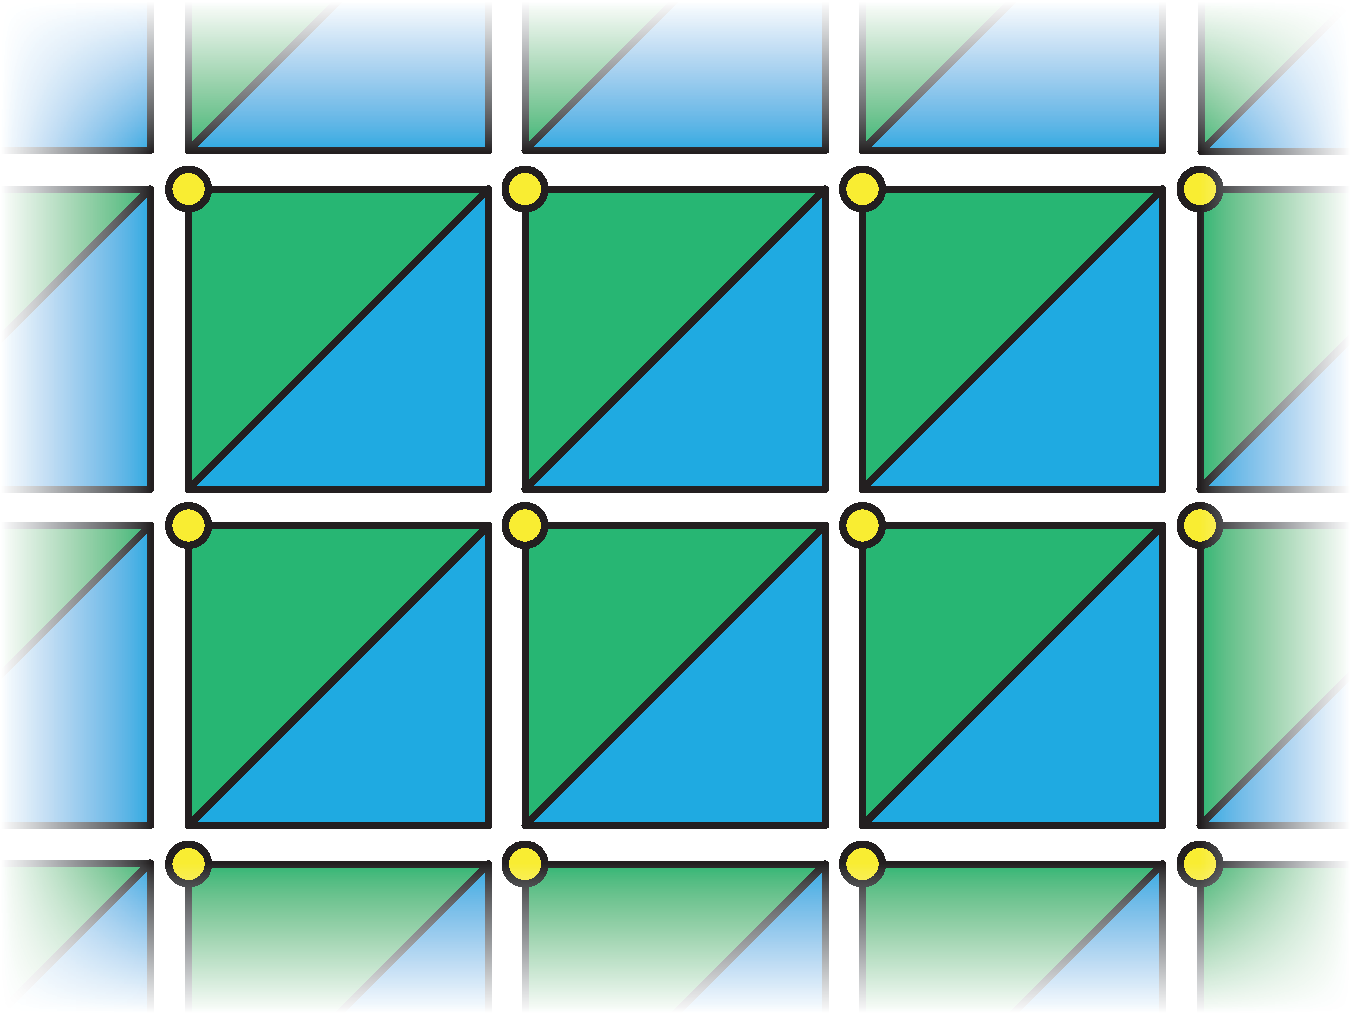
\includegraphics[width=0.6\textwidth]{images/bpa_point_triangle_ratio}
	\caption{
		Explanation for the ratio between mesh size and point cloud size approaching two.
		If the surface of an object and the corresponding points and triangles are completely unwrapped into a plane, each surface point may be associated with exactly two triangle.
	}
	\label{fig:bpa_point_triangle_ratio}
\end{figure}
%
This correlation now allows to calculate an approximation for the input raycasting resolution given a number of output triangles, which becomes handy if a triangle budget is specified for the output mesh.

The BPA timings in \cref{tbl:bpa_results}, especially at higher resolutions, further show that the algorithm's runtime is strongly related to the number of points of the cloud.
For each \SI{1}{\kilo\nothing} points, the BPA requires roughly \SI{4}{\milli\second} runtime, emitting \SI{2}{\kilo\nothing} triangles.
At lower resolutions, the overhead of the parallelization becomes visible, which is not as straight-forward as for the embarrassingly parallel tri-dexel or direct intersection, \cf the corresponding work \cite{bpa_vml}.

Concerning memory demands, the BPA requires quite a bit of space for its acceleration structure, a regular grid partitioning the point cloud.
This grid greatly speeds up the search for nearby points during pivoting.
Furthermore, this grid is also the basis for a parallelization, \cf the corresponding work for details \cite{bpa_vml}.
In addition to the grid, the currently built mesh is stored in a rich data structure, maintaining not only triangles but also a lot of connectivity information between vertices, edges and faces.
These data structures sum up to roughly \SI{1.2}{\gibi\byte} memory during a reconstruct of the impeller at a resolution of 400.

\Cref{fig:bpa_results} shows renderings of the result meshes after running the VML's BPA on point clouds created with a resolution of 400.
%
\begin{figure}
	\centering
	\begin{subfigure}[b]{0.34\textwidth}
		\centering
		\includegraphics[width=\textwidth]{bpa_cube2}
		\caption{cube2}
		\label{fig:bpa_cube2}
	\end{subfigure}
	\hspace{1cm}
	\begin{subfigure}[b]{0.34\textwidth}
		\centering
		\includegraphics[width=\textwidth]{bpa_cylinder_head}
		\caption{cylinder\_head}
		\label{fig:bpa_cylinder_head}
	\end{subfigure}
	\begin{subfigure}[b]{0.34\textwidth}
		\centering
		\includegraphics[width=\textwidth]{bpa_cylinders}
		\caption{cylinders}
		\label{fig:bpa_cylinders}
	\end{subfigure}
	\hspace{1cm}
	\begin{subfigure}[b]{0.34\textwidth}
		\centering
		\includegraphics[width=\textwidth]{bpa_cylinders_d}
		\caption{cylinders\_d}
		\label{fig:bpa_cylinders_d}
	\end{subfigure}
	\begin{subfigure}[b]{0.34\textwidth}
		\centering
		\includegraphics[width=\textwidth]{bpa_hq_impeller}
		\caption{impeller}
		\label{fig:bpa_hq_impeller}
	\end{subfigure}
	\hspace{1cm}
	\begin{subfigure}[b]{0.34\textwidth}
		\centering
		\includegraphics[width=\textwidth]{bpa_hq_impeller_2}
		\caption{impeller\_2}
		\label{fig:bpa_hq_impeller_2}
	\end{subfigure}
	\begin{subfigure}[b]{0.33\textwidth}
		\centering
		\includegraphics[width=\textwidth]{bpa_turbine}
		\caption{turbine}
		\label{fig:bpa_turbine}
	\end{subfigure}
	\caption{
		Renderings of the result meshes after applying the BPA reconstruction approach on a point cloud created with a resolution of 400 on the selected test scenes in \cref{tbl:test_scenes}.
	}
	\label{fig:bpa_results}
\end{figure}
%
All scenes except the turbine have been extracted without errors.
The BPA did a good job in creating a mesh for each point cloud, although the reconstructions are not perfect.
Especially sharp edges and corners are missing in all reconstructions.
Furthermore, similar to the tri-dexel, the BPA also produces a high number of triangles in flat regions, where far less triangles would be needed to express the same surface.
Again, this may be solved by running a post processing step which recombines adjacent triangles with equal normals.

Similar to the tri-dexel, the BPA also reproduces the original triangulation of the volumes in the cylinders\_d scene, clearly seen at the drilling and the lateral surface of the stock in \cref{fig:bpa_cylinders_d}.
Also the small rills between the blades of the impeller become visible again.
Although the tri-dexel does a slightly better job with these nuances, as it may calculate feature and apex points from the normals of its dexel nodes.
The BPA does not use point normals for reconstructing features, although a post processing pass might \eg further bend/tessellate created triangles based on their vertex normals.

Consequently, the only difficulty of the BPA is reconstructing small features, both convex and concave.
\Cref{fig:bpa_cylinder_head_edges} shows several concave and convex edges of the cylinder\_head scene which were not correctly reconstructed.
%
\begin{figure}
	\centering
	\begin{subfigure}[b]{0.49\textwidth}
		\centering
		\includegraphics[width=\textwidth]{bpa_cylinder_head_edges}
		\caption{cylinder\_head edges}
		\label{fig:bpa_cylinder_head_edges}
	\end{subfigure}
	\begin{subfigure}[b]{0.49\textwidth}
		\centering
		\includegraphics[width=\textwidth]{bpa_cylinder_head_thin_fin}
		\caption{cylinder\_head drilling at fin}
		\label{fig:bpa_cylinder_head_thin_fin}
	\end{subfigure}
	\caption{
		Details of the cylinder\_head scene.
		The meshes have been extracted using the BPA approach with a resolution of 400.
	}
	\label{fig:bpa_cylinder_head_details}
\end{figure}
%
Concerning concave features, the ball size is the BPA's limiting component as it does not allow the created surface to \enquote{crawl} into the sharp corners.
These features are simply rolled over.
Fine convex and concave features are only reconstructible from the normals of the point cloud and therefore ignored by the BPA.
Only geometry for which points are present in the point cloud is reconstructed by the BPA.
Surprisingly, due to the BPA's sole concentration on points, thin convex features such as the drilling at a fin of the cylinder\_head, \cf \cref{fig:bpa_cylinder_head_thin_fin}, are reconstructed quite robustly.
This part of the scene challenges the tri-dexel approach much more, as the cells almost collapse along one axis during slicing.

The turbine scene looks reasonable from a distance, \cf \cref{fig:bpa_turbine}.
However, the BPA has a hard time reconstructing the concave grooves, failing horribly at lower resolutions.
\Cref{fig:bpa_grooves} shows the turbine's grooves reconstructed from point clouds with various resolutions.
%
\begin{figure}
	\centering
	\begin{subfigure}[b]{0.24\textwidth}
		\centering
		\includegraphics[width=\textwidth]{bpa_turbine_groove_50}
		\caption{50}
		\label{fig:bpa_turbine_groove_50}
	\end{subfigure}
	\begin{subfigure}[b]{0.24\textwidth}
		\centering
		\includegraphics[width=\textwidth]{bpa_turbine_groove_100}
		\caption{100}
		\label{fig:bpa_turbine_groove_100}
	\end{subfigure}
	\begin{subfigure}[b]{0.24\textwidth}
		\centering
		\includegraphics[width=\textwidth]{bpa_turbine_groove_200}
		\caption{200}
		\label{fig:bpa_turbine_groove_200}
	\end{subfigure}
	\begin{subfigure}[b]{0.24\textwidth}
		\centering
		\includegraphics[width=\textwidth]{bpa_turbine_groove_400}
		\caption{400}
		\label{fig:bpa_turbine_groove_400}
	\end{subfigure}
	\caption{
		Detailed renderings with the same perspective of a groove of the turbine scene.
		The meshes were created using the BPA reconstruction algorithm run on a point cloud with the resolutions 50, 100, 200 and 400.
	}
	\label{fig:bpa_grooves}
\end{figure}
%
At a resolution of 50, the grooves are simply too small for the ball to roll inside.
Compared with the tri-dexel approach using the same resolution, which succeeds in recreating the groove, the BPA's result is terrible.
Increasing the resolution to 100 allows the ball to slip inside the groove, although still a lot of geometry is created spanning it.
At a resolution of 200, the groove becomes clearly visible.
However, the concave indentations at the groove's sides are still captured badly, especially the indentation at the bottom.
Finally, at a resolution of 400 the groove is reconstructed almost correctly, which only a few artifacts at the bottom.
Compared again with the tri-dexel results for the turbine's grooves, \cf \cref{fig:td_grooves}, the BPA requires approximately twice the resolution for a similar visual quality.

A further problem of the BPA is its instability inside concave features which are slightly larger than the ball as well as the possibility of the ball to roll inside the point cloud.
\Cref{fig:bpa_issues} shows cases for these two problems.
%
\begin{figure}
	\centering
	\begin{subfigure}[b]{0.49\textwidth}
		\centering
		\includegraphics[width=\textwidth]{bpa_cylinder_head_non_manif}
		\caption{cylinder\_head 50}
		\label{fig:bpa_cylinder_head_non_manif}
	\end{subfigure}
	\begin{subfigure}[b]{0.49\textwidth}
		\centering
		\includegraphics[width=\textwidth]{bpa_turbine_inside}
		\caption{turbine 200}
		\label{fig:bpa_turbine_inside}
	\end{subfigure}
	\caption{
		Error in the cylinder\_head and turbine scene after BPA reconstruction.
		Boundary edges are marked in green.
	}
	\label{fig:bpa_issues}
\end{figure}

The left rendering, \cref{fig:bpa_cylinder_head_non_manif}, shows the creation of holes and non-manifold triangles between two fins of the cylinder\_head.
Such problems occur if the ball suddenly switches sides inside a concave feature, creating a triangle spanning the indentation.
Usually, the edges of these triangles cannot be pivoted further and remain boundaries.

The right rendering shows a cog of the turbine where the ball has fell inside the point cloud.
Between the differently oriented meshes, one created from outside, one from inside, lots of boundary edges and overlapping triangles are created.
If sufficient density of the point cloud is guaranteed, this case should, theoretically, never occur.
However, since all pivotings are subject to numeric calculations, there are indeed cases where the ball may still roll inside the point cloud.
Increasing the ball's size may help to minimize the likelihood of such an error, but comes at the cost of worse feature reconstruction.

Concerning the created boundary edges and holes, \cf \cref{tbl:bpa_boundary edges}, the BPA is quite robust if the point cloud does not contain concave features which are slightly larger than the size of the ball.
%
\begin{table}
	\centering
	\begin{tabular}{l|r|r|r|r}
		resolution     &  50 &  100 &  200 &  400 \\
		\midrule
		cube2          &   0 &    0 &    0 &    0 \\
		cylinders\_d   &   0 &    0 &    0 &    0 \\
		cylinders      &   0 &    0 &    0 &    0 \\
		cylinder\_head & 110 &    0 &    0 &    0 \\
		impeller       &   0 &    0 &    0 &    0 \\
		impeller\_2    &   0 &    0 &    0 &    0 \\
		turbine        &   0 & 3055 & 1721 & 3293 \\
	\end{tabular}
	\caption{
		Created boundary edges by the BPA surface extraction.
	}
	\label{tbl:bpa_boundary edges}
\end{table}
%
The only point clouds where boundary edges have been generated are the cylinder\_head, at a resolution of 50, and all turbine clouds higher than 50.

In all of these cases, the ball rolls inside a concave feature/hole and creates triangles spanning the sides of the feature, \cf \cref{fig:bpa_cylinder_head_non_manif,fig:bpa_turbine_groove_100}.
These cases could be resolved by analyzing the created mesh, finding non-manifold vertices/edges, removing affected triangles and rerunning the BPA on the remaining holes, maybe with different ball sizes.
If sufficient memory is available, the point cloud resolution may also be increased which allows the ball to be smaller and have more space to pivot in such small features.

In the turbine cases, the ball also frequently rolls inside the point cloud, even if it is only for smaller regions.
At the border of these regions, the mesh orientation changes and usually causes boundary edges to be left, as the BPA is not allowed to attach new triangles to existing triangles if they are differently orientated.
This kind of problem occurs primarily numerically and may only be mitigated by implementing further checks into the pivoting code.


Finally, to show the suitability of the point cloud for other algorithms outside the VML, a few renderings of the more complex scenes from meshes reconstructed with the Poisson reconstruction approach are discussed.
\Cref{fig:poisson_results} shows renderings of the cylinder\_head and impeller scene after applying the Poisson surface reconstruction filter available in MeshLab.
%
\begin{figure}
	\centering
	\begin{subfigure}[b]{0.49\textwidth}
		\centering
		\includegraphics[width=\textwidth]{poi_cylinder_head}
		\caption{cylinder\_head}
		\label{fig:poi_cylinder_head}
	\end{subfigure}
	\begin{subfigure}[b]{0.49\textwidth}
		\centering
		\includegraphics[width=\textwidth]{poi_cylinder_head_detail}
		\caption{cylinder\_head details}
		\label{fig:poi_cylinder_head_detail}
	\end{subfigure}
	\begin{subfigure}[b]{0.49\textwidth}
		\centering
		\includegraphics[width=\textwidth]{poi_hq_impeller}
		\caption{impeller}
		\label{fig:poi_hq_impeller}
	\end{subfigure}
	\begin{subfigure}[b]{0.49\textwidth}
		\centering
		\includegraphics[width=\textwidth]{poi_hq_impeller_points}
		\caption{impeller edges}
		\label{fig:poi_hq_impeller_points}
	\end{subfigure}
	\caption{
		Renderings of the cylinder\_head and impeller scenes of reconstructions using the Poisson surface reconstruction filter from MeshLab.
		The point cloud was created with a resolution of 400.
		The Poisson filter was parameterized with an octree depth of ten, solver divide at eight, one sample per node and a surface offsetting of one, \cf corresponding dialog in MeshLab.
	}
	\label{fig:poisson_results}
\end{figure}
%
As the Poisson algorithm tries to be robust against inhomogeneous and noisy inputs, sharp features are considered outliers and lost during the function fitting process.
This gives the reconstructed meshes a smooth and roundish appearance, as visible in the general renderings in \cref{fig:poi_cylinder_head,fig:poi_hq_impeller}.
The detailed rendering of a drilling of the cylinder\_head in \cref{fig:poi_cylinder_head_detail} further demonstrates the loss of sharp edges.
Additionally, the structure in the upper right, the drilling at the fin, is almost completely lost as the structure is too thin to allow the creation of a surface.

\Cref{fig:poi_hq_impeller_points} shows a reconstructed blade of the impeller together with the sampled point cloud.
The amount of lost volume, especially at the blade's tip and edge at the left, is clearly visible, as the surface only bends towards the points in flatter regions.
Nevertheless, the resulting triangulation is appealing with even a bit of adaptivity, containing larger triangles in flatter regions.
All runs of the algorithm generated manifold and closed meshes for all tested point clouds.

\Cref{fig:poi_grooves} shows a groove of the turbine reconstructed from point clouds with various resolutions.
%
\begin{figure}
	\begin{subfigure}[b]{0.24\textwidth}
		\centering
		\includegraphics[width=\textwidth]{poi_turbine_groove_50}
		\caption{50}
		\label{fig:poi_turbine_groove_50}
	\end{subfigure}
	\begin{subfigure}[b]{0.24\textwidth}
		\centering
		\includegraphics[width=\textwidth]{poi_turbine_groove_100}
		\caption{100}
		\label{fig:poi_turbine_groove_100}
	\end{subfigure}
	\begin{subfigure}[b]{0.24\textwidth}
		\centering
		\includegraphics[width=\textwidth]{poi_turbine_groove_200}
		\caption{200}
		\label{fig:poi_turbine_groove_200}
	\end{subfigure}
	\begin{subfigure}[b]{0.24\textwidth}
		\centering
		\includegraphics[width=\textwidth]{poi_turbine_groove_400}
		\caption{400}
		\label{fig:poi_turbine_groove_400}
	\end{subfigure}
	\caption{
		Detailed renderings with the same perspective of a groove of the turbine scene.
		The meshes were created using the Poisson surface reconstruction filter of MeshLab run on a point cloud with the resolutions 50, 100, 200 and 400.
	}
	\label{fig:poi_grooves}
\end{figure}
%
At a resolution of 50, the groove is simply sampled too poor for the Poisson reconstruction to create the indentation.
This result is comparable to the BPA's performance at the same resolution in \cref{fig:bpa_turbine_groove_50}, where the ball was too big to roll inside the groove.
At a resolution of 100, the groove becomes visible as the indentation is created.
Still, the concave rills inside the notch as well as the indentation at the bottom of the groove are not visible yet.
The rills are acceptably reconstructed at a resolution of 200 while the bottom notch requires a resolution of 400 to appear.
Compared with the tri-dexel approach and similarly to the BPA, the Poisson surface reconstruction also requires roughly twice the resolution of the tri-dexel for a visually comparable output regarding the captured features.
However, as detailed in \cref{sec:point_cloud_concept}, the main reason for this issue is the richer semantic carried by the tri-dexel image when compared with a point cloud.

Concerning timings, the Poisson surface reconstruction filter of MeshLab is roughly 10 - 20 times slower than the BPA implementation of the VML, \cf \cref{tbl:bpa_results}.
The runtimes for the turbine scene, for example, at the resolutions 50, 100, 200 and 400, averaged over five runs, are \SI{941}{\milli\second}, \SI{2816}{\milli\second}, \SI{10587}{\milli\second} and \SI{46397}{\milli\second}, respectively, measured using MeshLab.
However, the algorithm employed by MeshLab runs single threaded.
Accounting for this difference, MeshLab's Poisson implementation and the VML's BPA would both require a runtime in the same order of magnitude
During the reconstruction at resolution 400, roughly \SI{400}{\mebi\byte} were allocated, making the Poisson algorithm significantly more light-weight than the BPA.

Similar to the external Poisson surface reconstruction algorithm of MeshLab, any other external algorithm may be run on the point clouds created from the raycaster in \cref{sec:point_cloud_implementation}.
MeshLab for example further offers an implementation of alpha shapes \cite{alpha_shape}, an own BPA, two marching cubes variants based on MLS \cite{meshlab_mc_mls_1, meshlab_mc_mls_2} as well as an algorithm based on distance fields from the VCG library \cite{vcg}.
Further libraries for point cloud surface reconstruction include the Computational Geometry Algorithms Library (CGAL) \cite{cgal}, the Visualization Toolkit (VTK) \cite{vtk}, QHull \cite{qhull} or the Point Cloud Library (PCL) \cite{pcl}.
